\section{Istruzione utilizzo utente operatore}
La seguente sezione fornirà indicazioni utili per il corretto utilizzo del software nel caso l'utente interessato sia l'operatore che deve guidare l'unità.

\subsection{Guida automatica dell'unità}
\begin{itemize}
    \item Premere sul pulsante "Start" per iniziare il movimento del muletto verso il primo POI della lista;
    \item i movimenti effettuati sono visualizzati nella mappa e nelle frecce.
    
\end{itemize}
\begin{figure}[H]
    \centering
    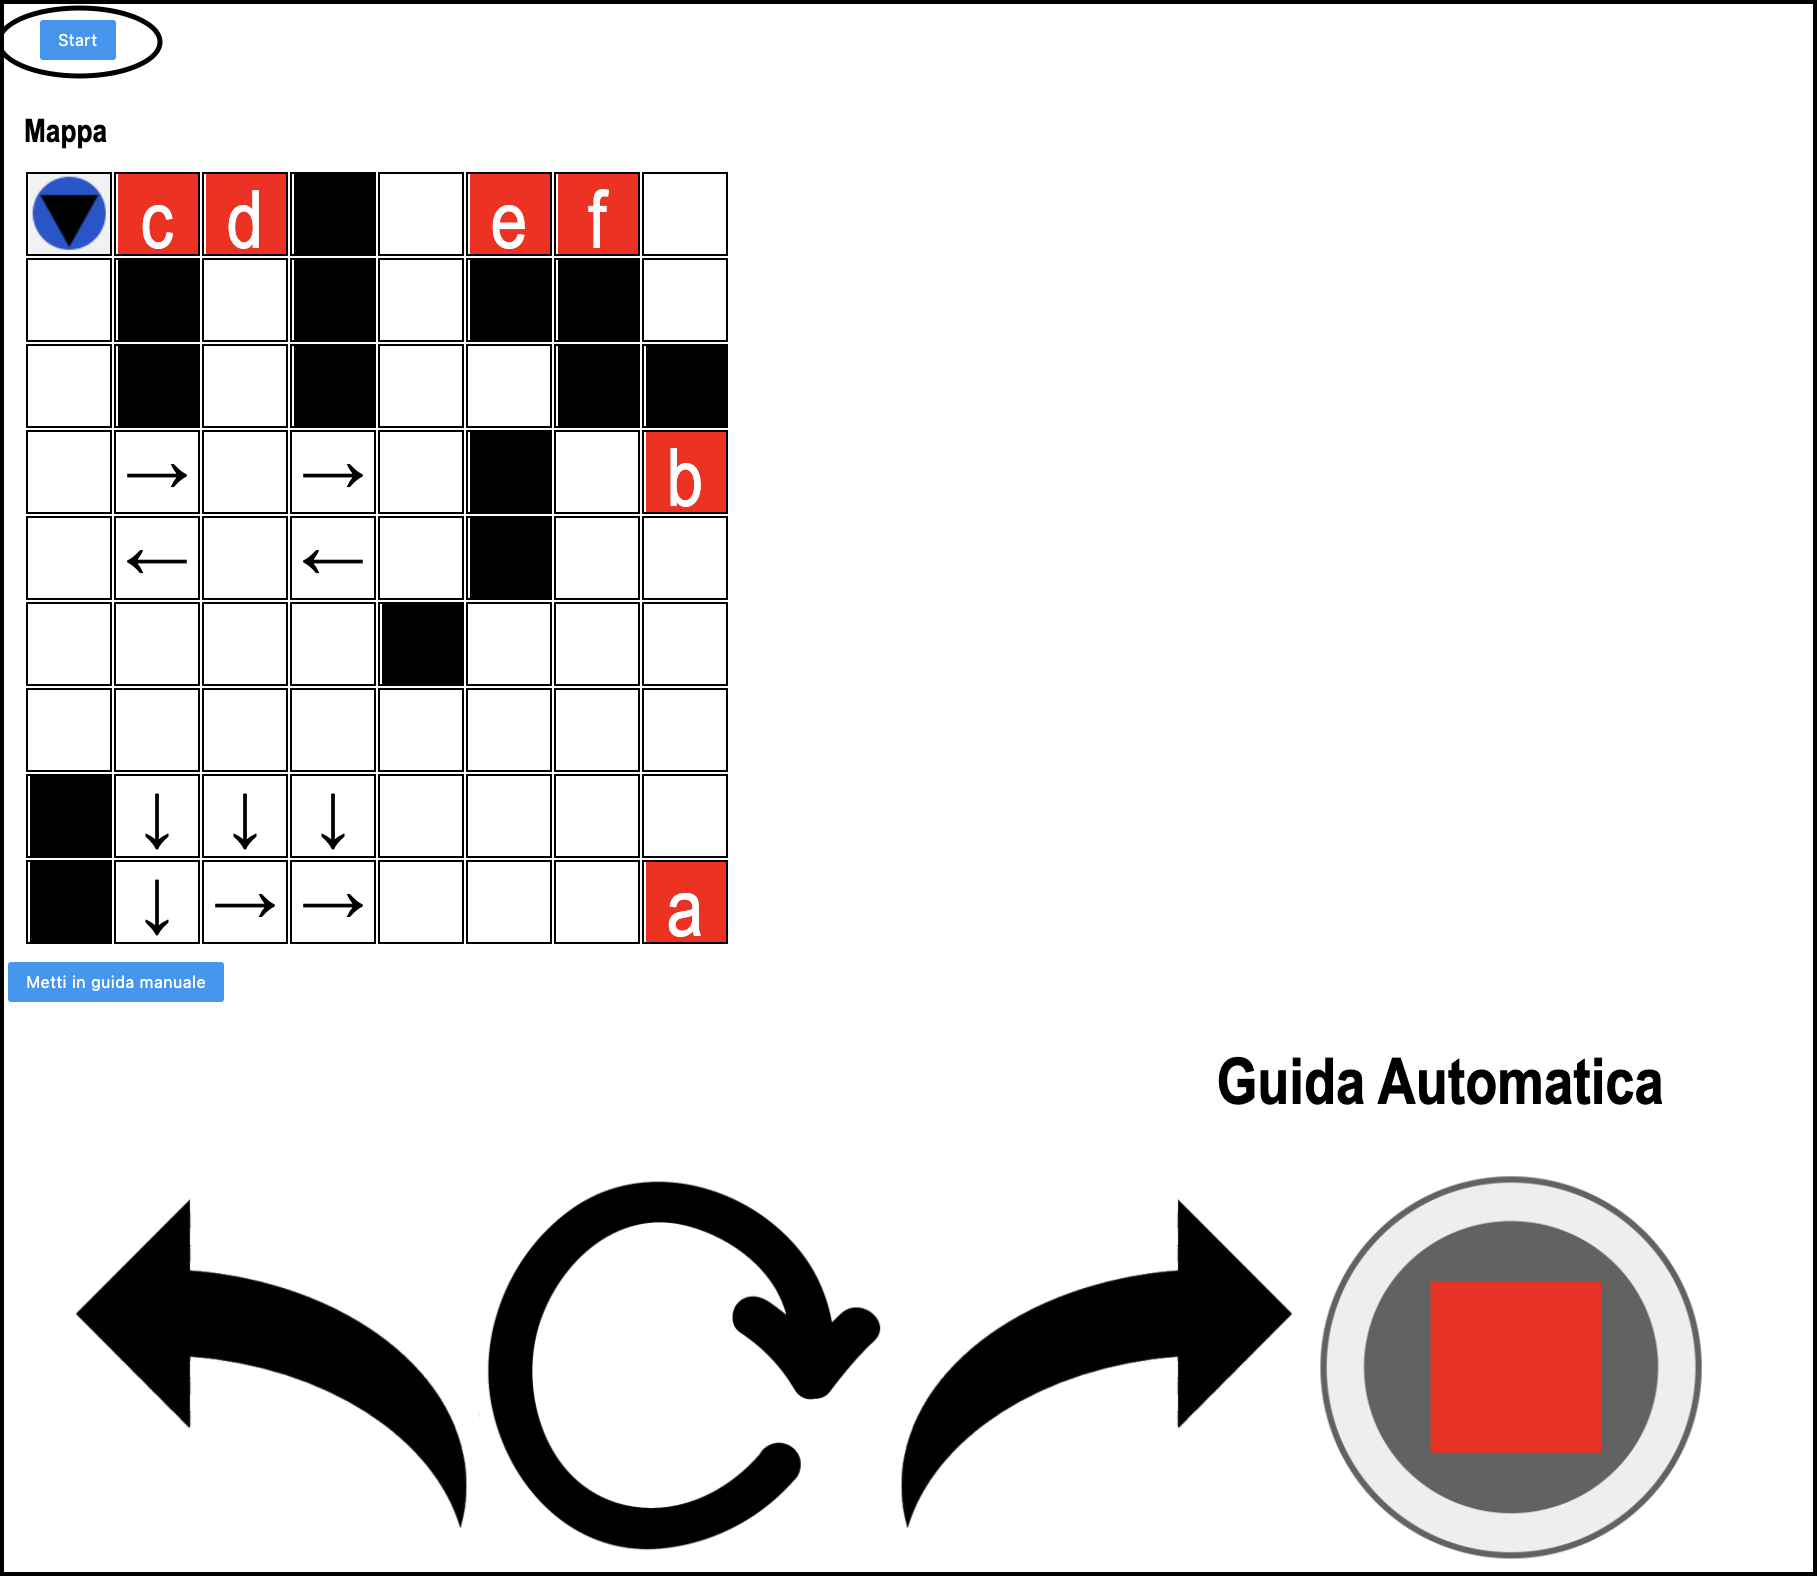
\includegraphics[scale=0.45]{res/images/forklift_start.png}
    \caption{Schermata guida automatica dell'unità}
\end{figure}
\pagebreak
\subsection{Passaggio a guida manuale/automatica}
\begin{itemize}
    \item Premere sul pulsante "Cambio guida";
    \item i comandi verranno cambiati in base allo stato di guida;
\end{itemize}
\begin{figure}[H]
    \centering
    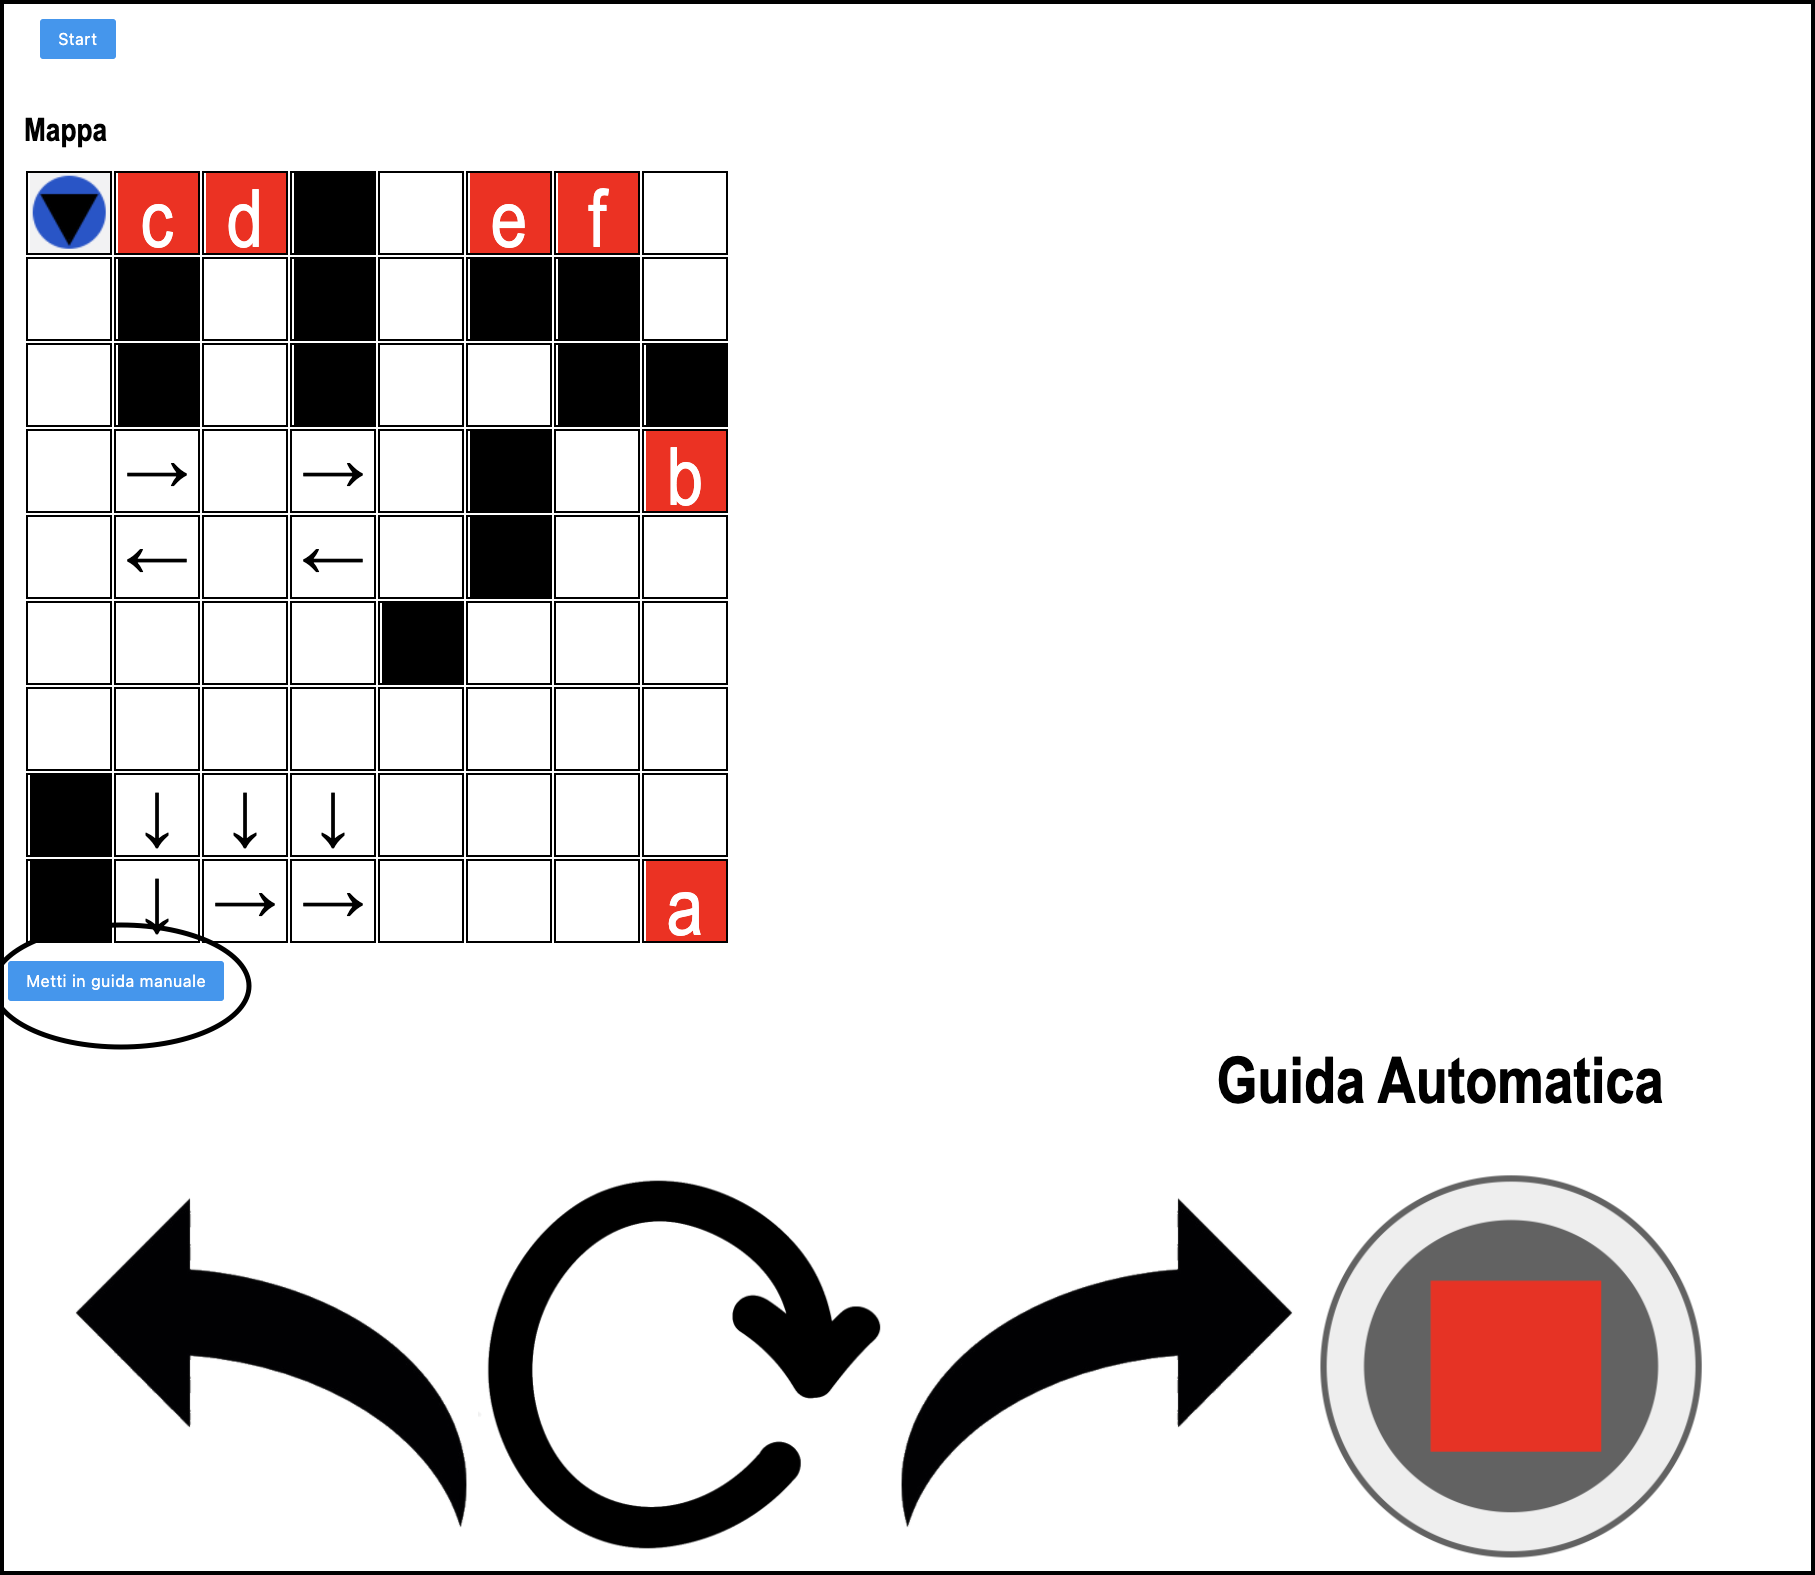
\includegraphics[scale=0.45]{res/images/forklift_cambioguida.png}
    \caption{Schermata passaggio a guida manuale/automatica}
\end{figure}
\pagebreak

\subsection{Guida manuale dell'unità}
\begin{itemize}
    \item Premere sul pulsante "Metti in guida manuale";
    \item premere "Start" per iniziare il movimento del muletto;
    \item premere nella frecce visualizzate per spostare l'unità nella direzione desiderata;
    \item premere "Stop" per fermarsi;
\end{itemize}
\begin{figure}[H]
    \centering
  	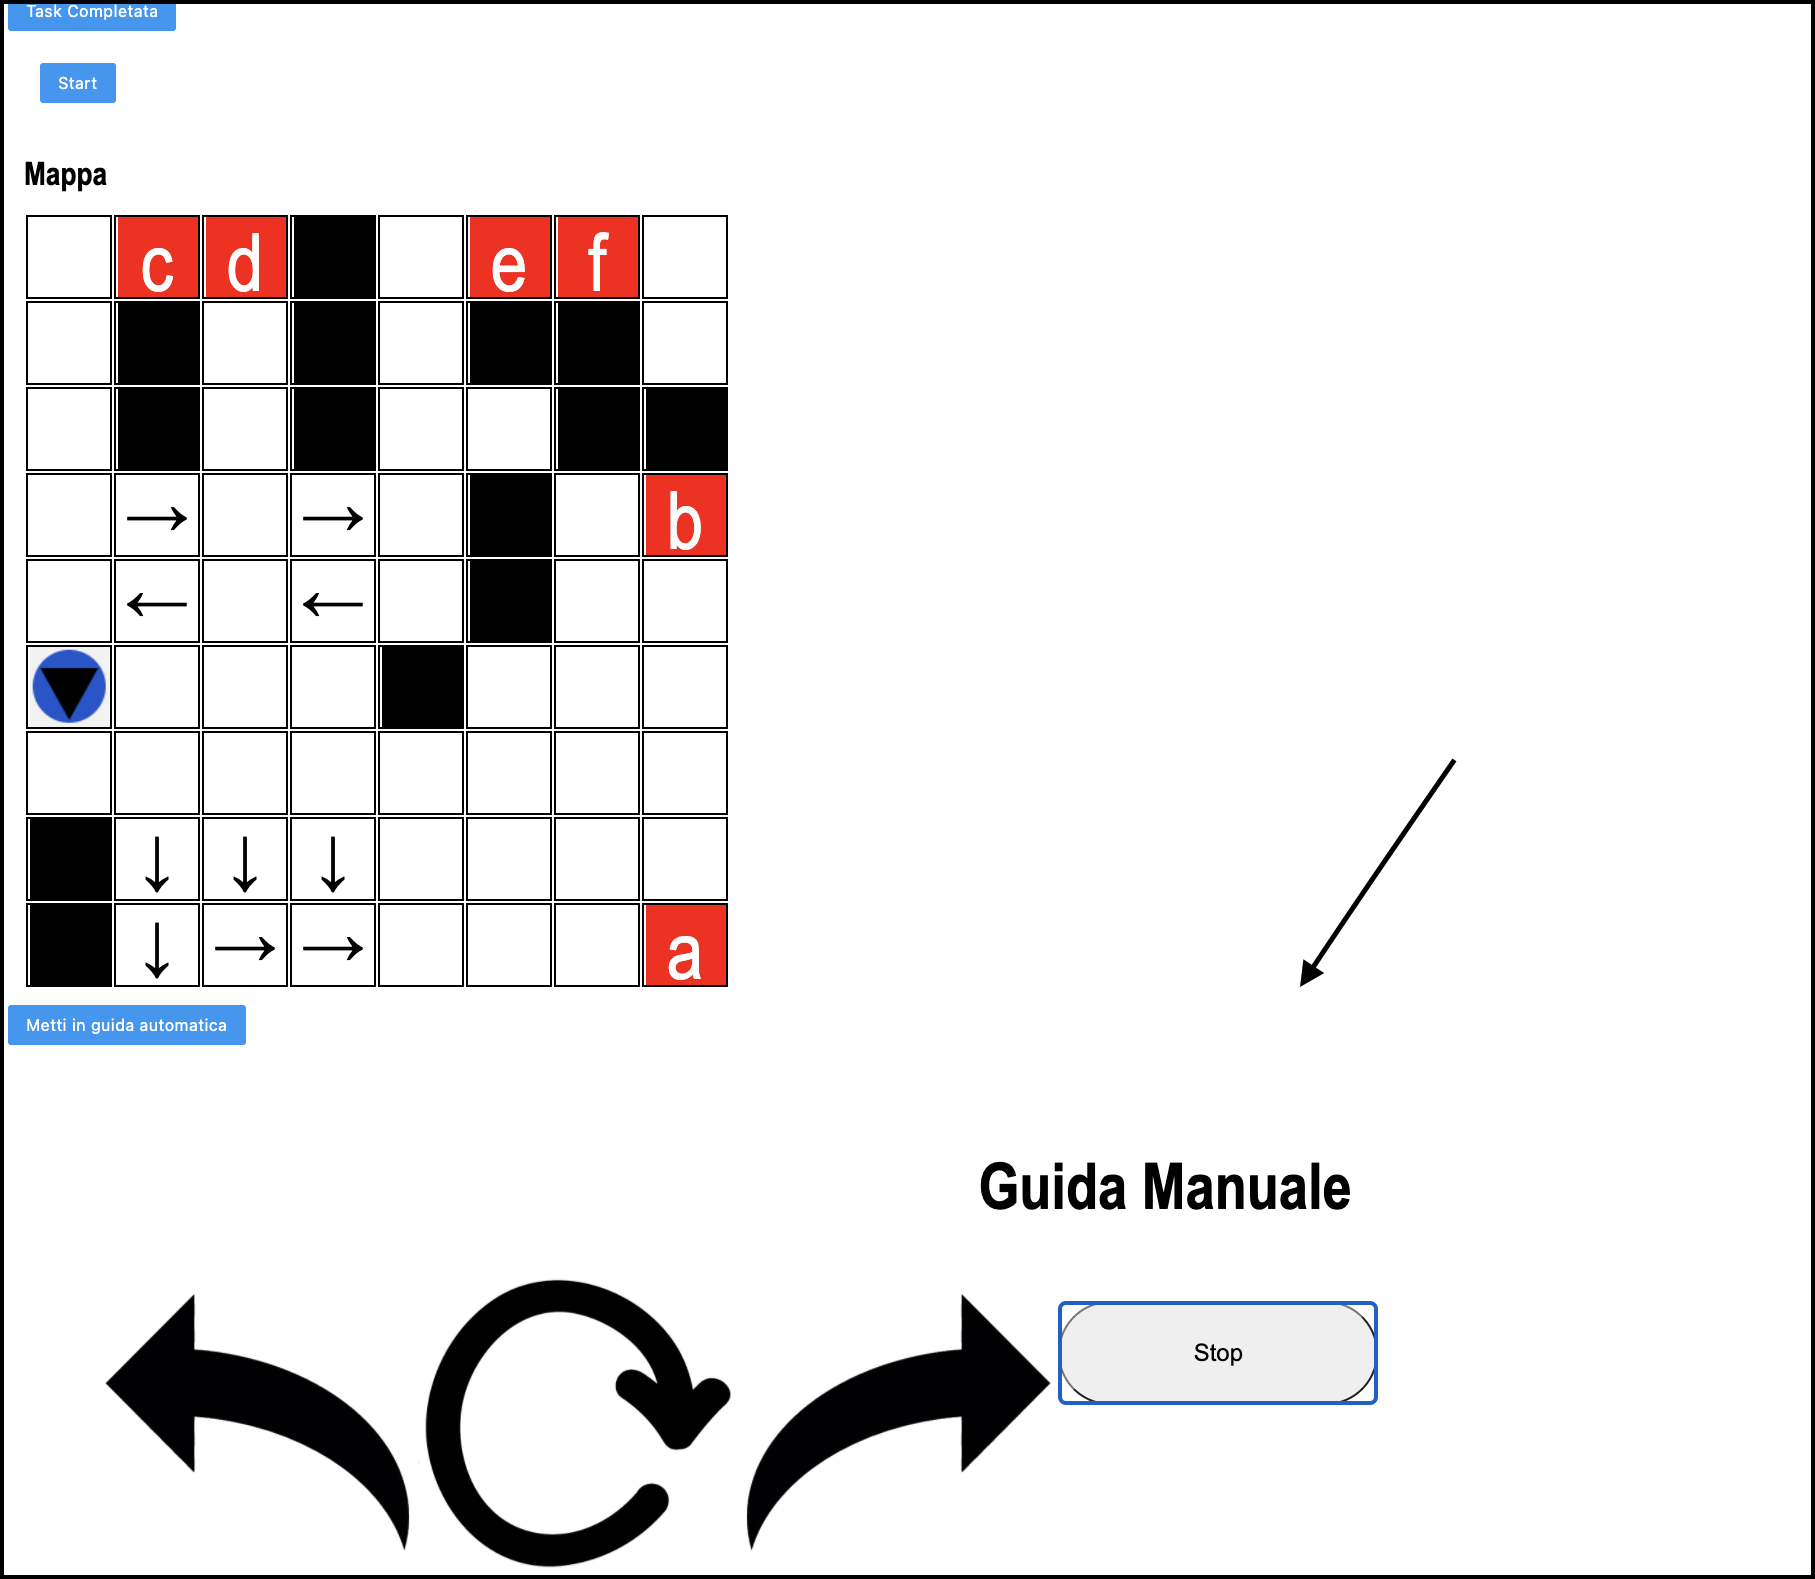
\includegraphics[scale=0.45]{res/images/forklift_guidamanuale.png}
  	\caption{Schermata guida manuale dell'unità}
\end{figure}
\pagebreak

\subsection{Completamento task}
\begin{itemize}
    \item Una volta raggiunto il POI, l'unità si ferma e viene visualizzato un pulsante "Task completata";
    \item premere su esso per notificare lo scarico delle merci e per continuare il proprio percorso.
\end{itemize}
\begin{figure}[H]
    \centering
    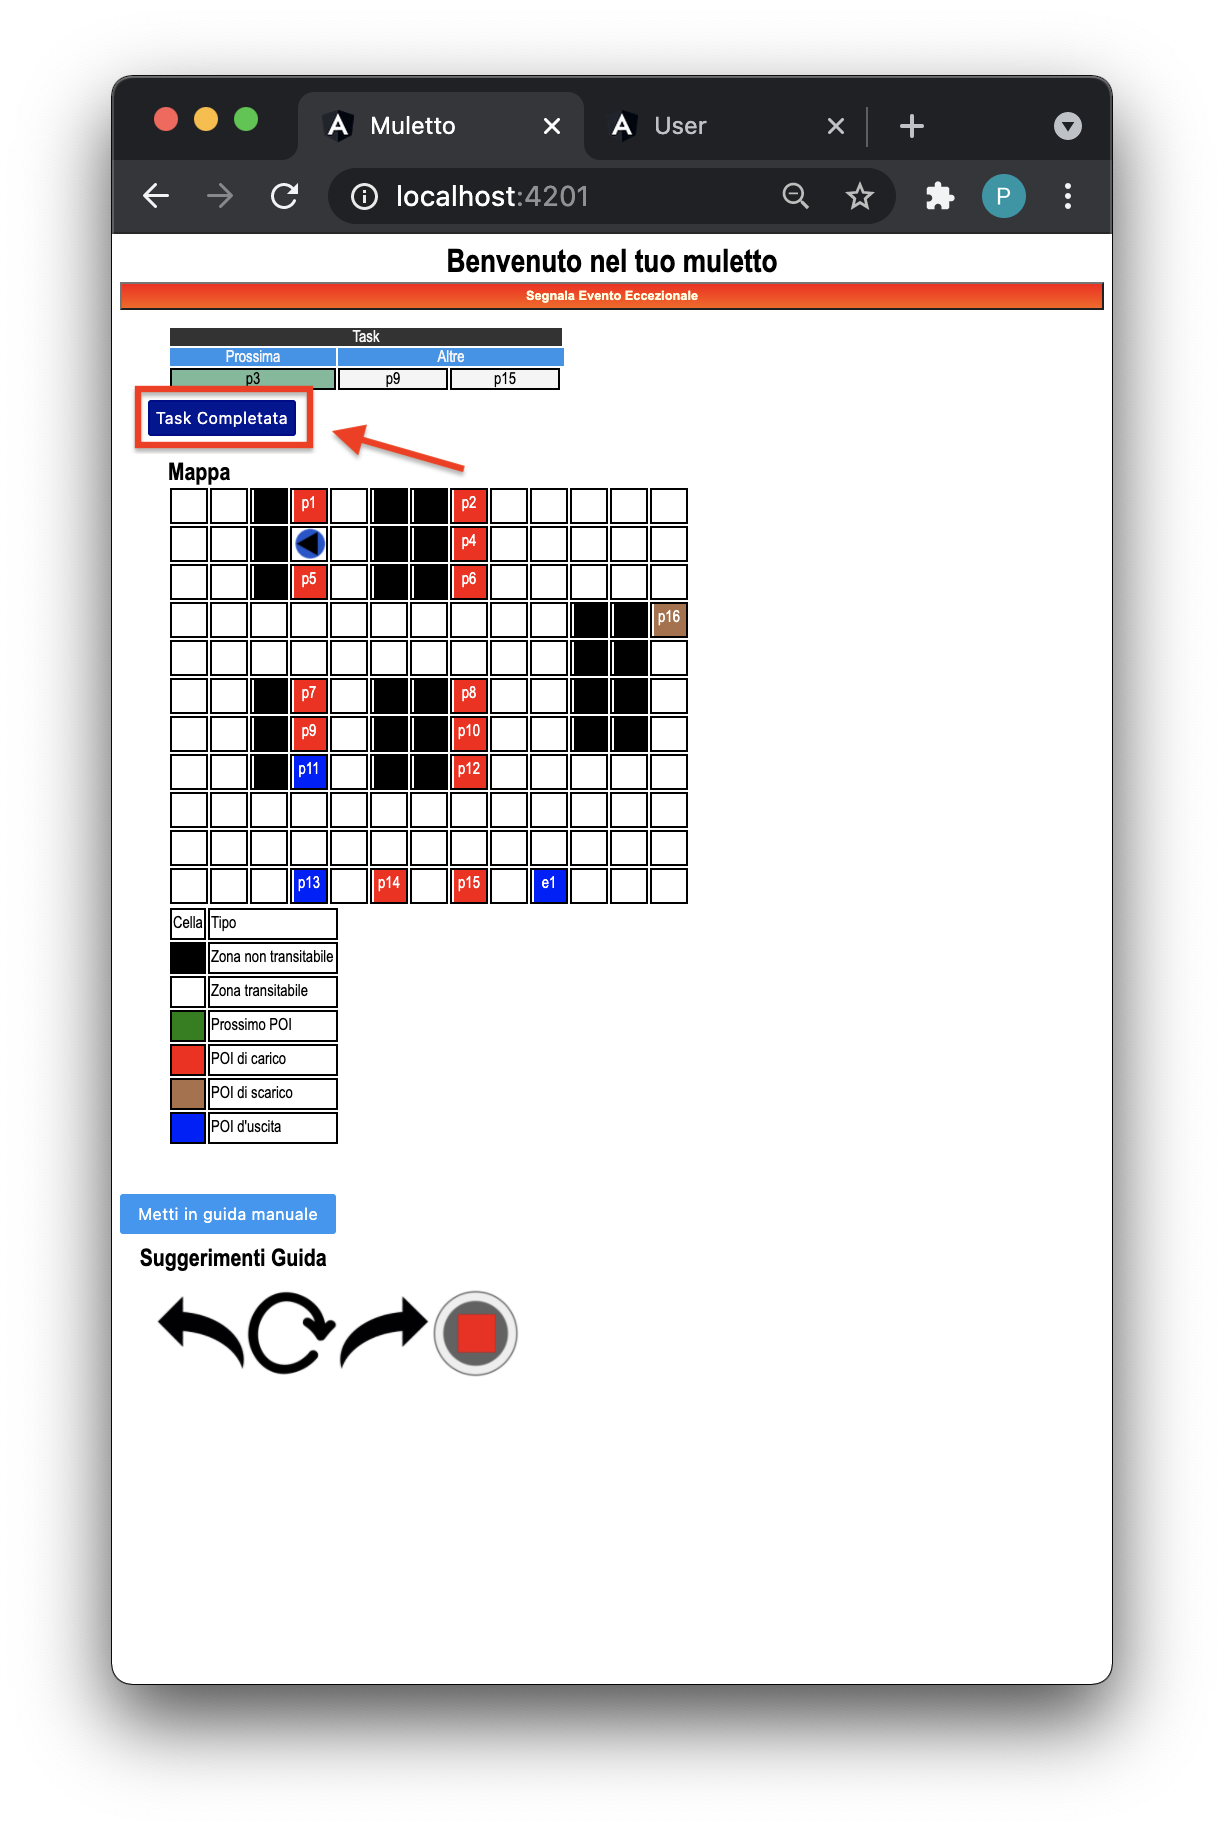
\includegraphics[scale=0.45]{res/images/forklift_taskcompletata.png}
\end{figure}
\pagebreak
\subsection{Segnalazione evento eccezionale}
\begin{itemize}
    \item Premere sul pulsante "Evento eccezionale" per notificare all'amministratore l'avvenimento di un evento non previsto.
\end{itemize}
\begin{figure}[H]
    \centering
    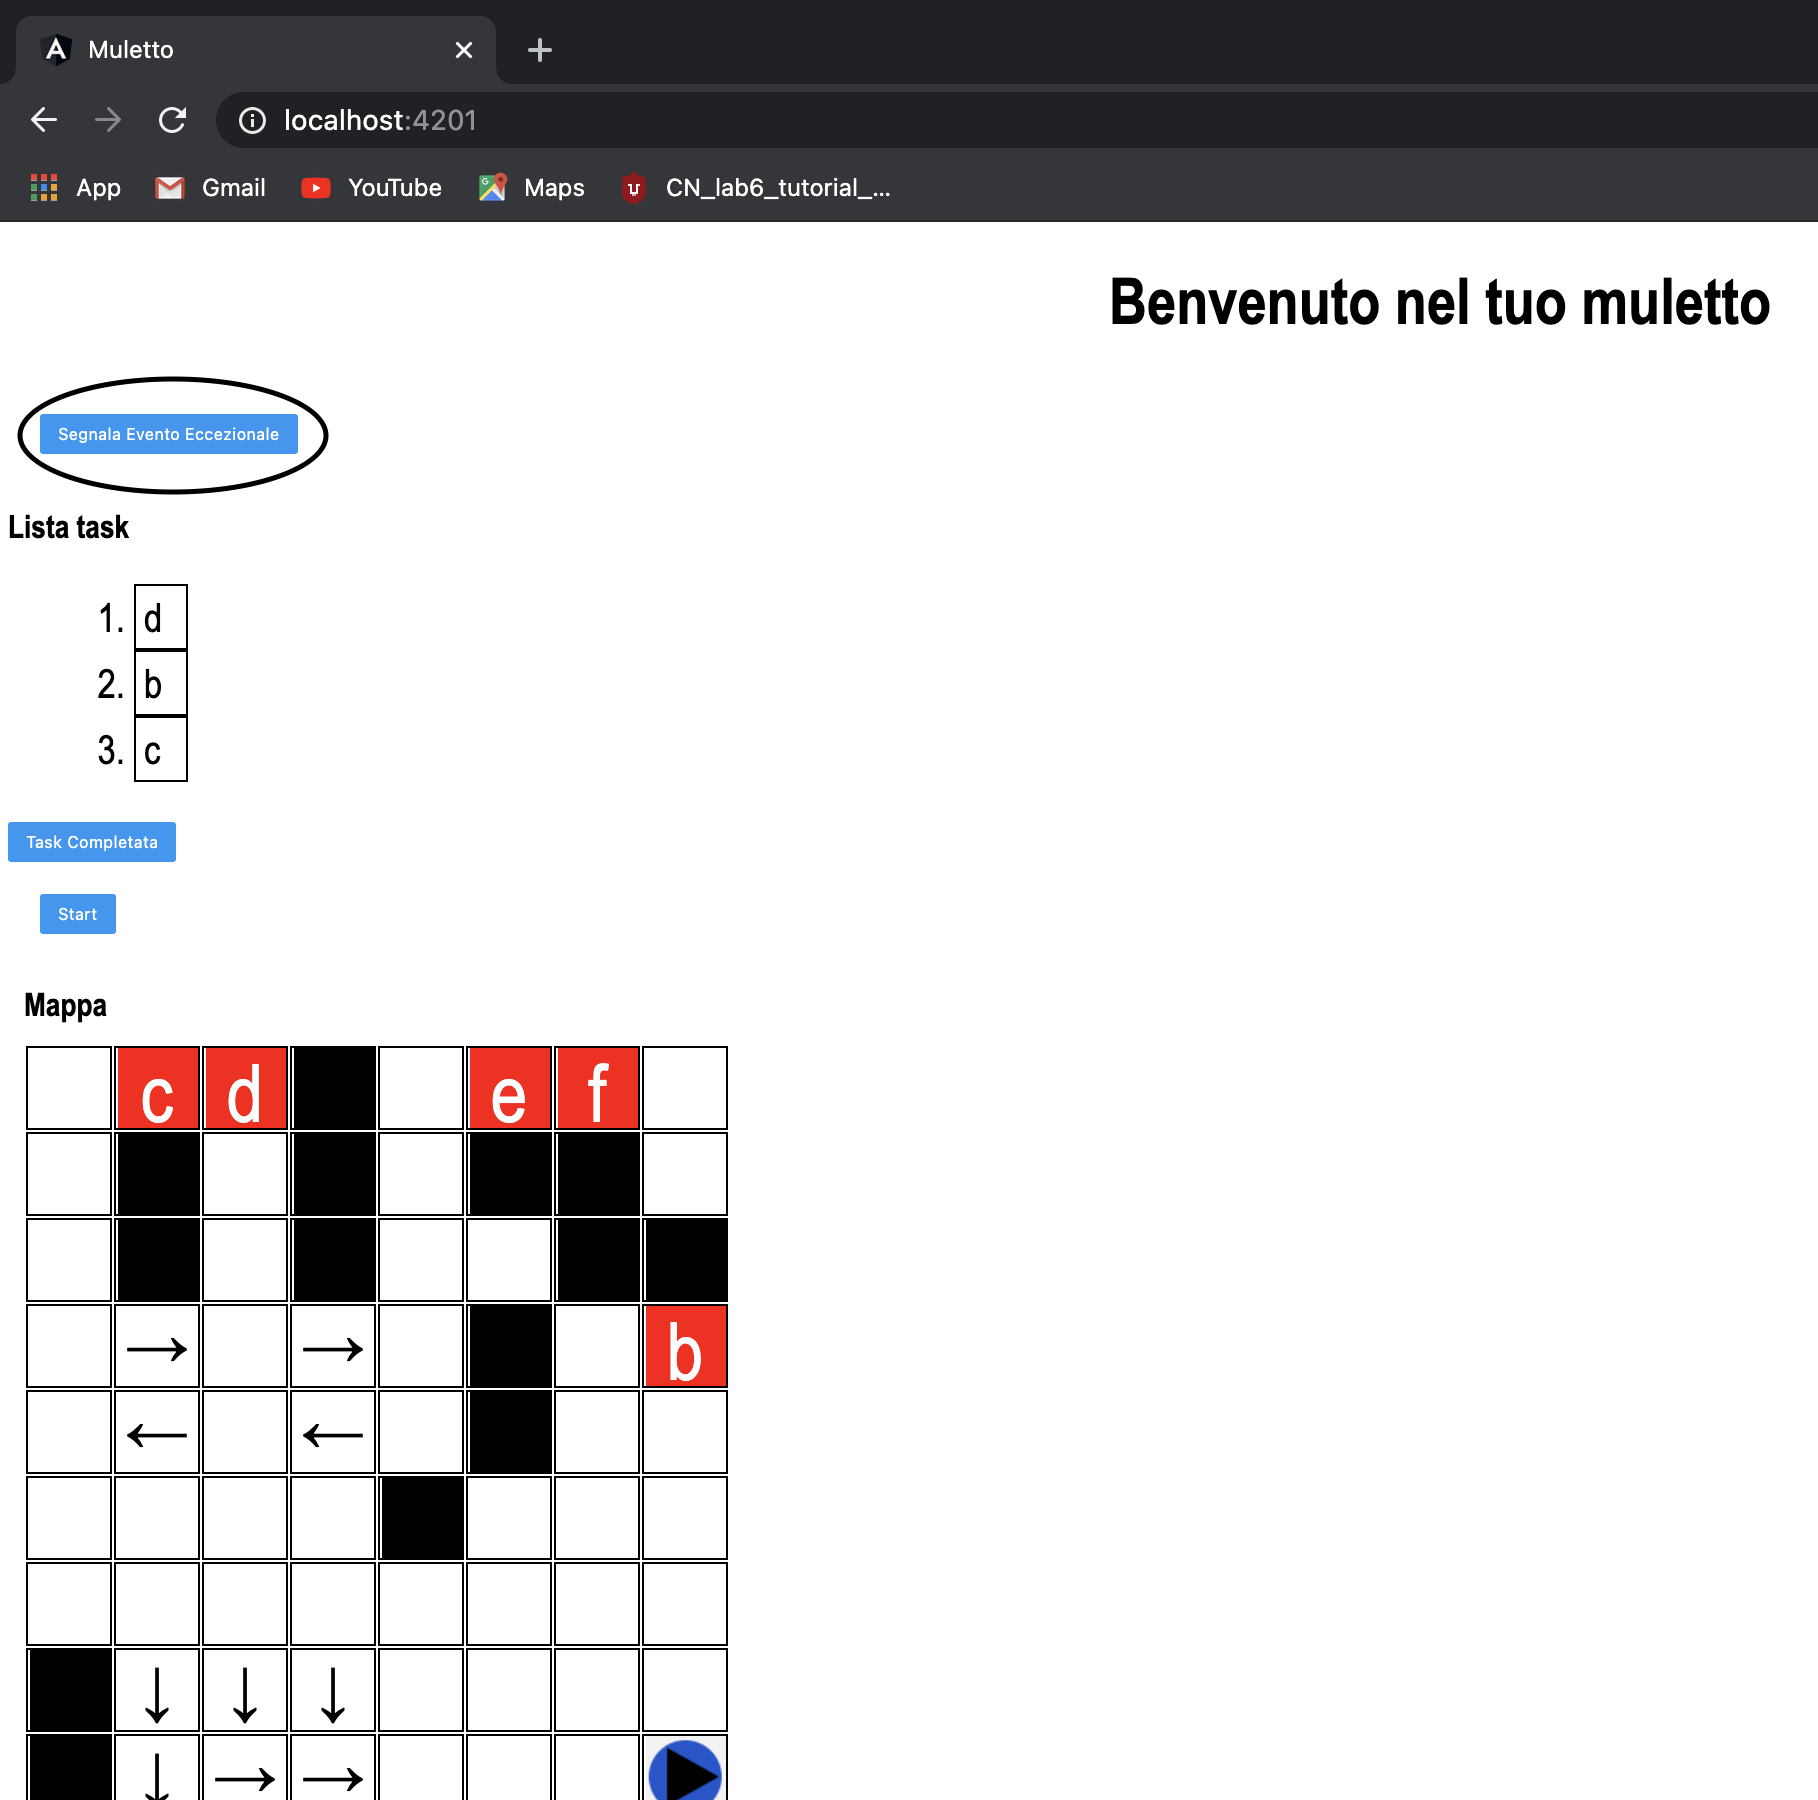
\includegraphics[scale=0.45]{res/images/forklift_evento.png}
    \caption{Schermata segnalazione evento eccezionale}
\end{figure}